\chapter{Background}\label{ch:background}

The following sections provide an overview of the main concepts and technologies that are relevant to the work presented in this thesis.

\section{Digital Twins}

A \acrfull{dt} is a physical and/or virtual machines or computer-based model that simulate, emulate, mirror, or ``twin'' the life of a physical entity, which may be an object, a process, a human, or a human-related feature \parencite{barricelliMultiModalApproachCreating2022}.

Far from a passive copy, a \acrshort{dt} is an intelligent and adaptive entity, acting as the living counterpart to its physical twin~\parencite{grievesDigitalTwinManufacturing2015,kritzingerDigitalTwinManufacturing2018}. It continuously monitors, analyzes, and optimizes the real-world process or object throughout its lifecycle~\parencite{negriReviewRolesDigital2017}. This not only allows for proactive maintenance and prevention of issues like defects and failures, but also enables experimentation and optimization through simulations of new configurations. The twinning process is allowed by the dynamic interplay between the digital twin, its physical counterpart, and the surrounding environment --- a continuous loop of interaction, communication, and refinement.

The \acrshort{dt} maintains continual awareness of its physical counterpart and surrounding environment through real-time data streams and extensive data storage capabilities. Descriptive data exchanges, facilitated by big data infrastructure, ensure consistent synchronization with the physical system. Advanced algorithms, including data fusion, big data analytics, and \acrshort{ai}-based descriptive methods, are applied to extract valuable insights from this rich data pool. The modular and highly parameterized architecture of the \acrshort{dt} enables rapid reconfiguration, allowing it to evolve alongside its physical twin. This synchronization ensures the \acrshort{dt} constantly reflects the properties and changes occurring in the real world.

Leveraging its \acrshort{ai} capabilities, the \acrshort{dt} transcends mere emulation by uncovering hidden patterns, unknown correlations, and comprehensive system descriptions. This holistic understanding of the physical system, combined with the ability to record, control, and monitor its condition, enables techniques for failure forecasting, simulation of potential solutions, and even activation of self-healing mechanisms. This powerful combination facilitates a predictive maintenance approach, where proactive interventions prevent failures and optimize performance through simulated testing and solution selection.

Despite their inherent intelligence, \acrshort{dt}s are not designed to operate in complete autonomy. \acrshort{ai}-based applications and \acrshort{dt}s often require significant human intervention, particularly when testing novel features and modifications on physical assets, as well as when the systems are leveraged to provide crucial outputs like medical diagnoses and treatment recommendations~\parencite{barricelliSurveyDigitalTwin2019}.

\subsection{Historical Notes}

The concept of \acrshort{dt} first appeared in the field of \acrfull{plm}, where it was informally introduced in 2002 by Michael Grieves, and formalized in later works \parencite{grievesDigitalTwinManufacturing2015,grievesDigitalTwinMitigating2017}. Grieves' \acrshort{dt} model, represented in Figure~\ref{fig:grieves_digital_twin} was composed by three primary elements:
\begin{enumerate}
    \item A real space containing a physical object;
    \item A virtual space containing a virtual object;
    \item The link for data flow from real space to virtual space (and virtual sub-spaces), and for information flow from virtual space (and sub-spaces) to real space. This last element is the enabler of data exchange, thus allowing the convergence and synchronization of the virtual and physical systems.
\end{enumerate}

\begin{figure}
    \centering
    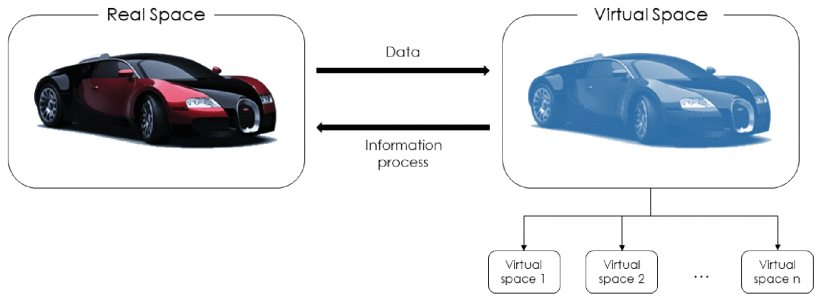
\includegraphics[width=0.8\textwidth]{images/dt_model_grieves.png}
    \caption[Grieves' digital twin model]{Grieves' digital twin model. From \cite{barricelliSurveyDigitalTwin2019}, \textit{Research Background} section, CC-BY 4.0 license.}
    \label{fig:grieves_digital_twin}
\end{figure}

A later development was proposed by \cite{framlingProductAgentsHandling2003}, who proposed ``an agent-based architecture where each product item has a corresponding virtual counterpart or agent associated with it''. Exploiting the seamless connection provided by the spread of Internet technologies, the envisioned agents should guarantee the synchronization with their physical counterpart, providing also services for them~\parencite{framlingProductAgentsHandling2003}. The authors' proposal is based on the consideration that an effective \acrshort{plm} system should always have access to a faithful view of the product status and information, from when it is planned and manufactured, through its time of use, and until the time of disposal.

Following Grieves' definition, \acrshort{dt}s garnered much interest in the aerospace and defense industries~\parencite{negriReviewRolesDigital2017}.
NASA researched \acrshort{dt}s as a way to reduce costs and resources for its space assets. Their investigation lead to a roadmap that confirmed the vale of \acrshort{dt}s in improving performance in the field of aviation. The authors defined the DT as ``an integrated multi-physics, multi-scale, probabilistic simulation of a vehicle or system that uses the best available physical models, sensor updates, fleet history, etc., to mirror the life of its flying twin. The digital twin is ultra-realistic and may consider one or more important and interdependent vehicle systems, including propulsion/energy storage, avionics, life support, vehicle structure, thermal management/TPS, etc.''~\parencite{shaftoModelingSimulationInformation2010}. The U.S. Air Force also developed the \acrfull{adt}, a computational model of individual aircrafts, which had the potential to improve the way U.S. Air Force aircrafts were managed over their entire lifecycle by creating individualized structural management plans~\parencite{tuegelAirframeDigitalTwin2012,gockelChallengesStructuralLife2012}.

Finally, \acrshort{dt}s also are key point of Industry 4.0~\parencite{brettelHowVirtualizationDecentralization2014,hermannDesignPrinciplesIndustrie2016,vachalekDigitalTwinIndustrial2017,negriReviewRolesDigital2017}, where they are used to monitor and optimize the performance of manufacturing systems, and to support the development of new products and services. The \acrshort{dt} is an enabler for the digital transformation of the manufacturing industry, and it is a fundamental component of the smart factory \parencite{mabkhotRequirementsSmartFactory2018}. 

\iffalse
    \subsection{Characteristics of Digital Twins}

    Seamless and reliable communication is fundamental to \acrshort{dt} functionality. Both physical and virtual twins require networking devices to facilitate continuous data exchange, achieved either through direct physical connections or indirect cloud-based networks. This facilitates a constant flow of information from the physical twin, which describes the physical twin status and change with time along its lifecycle, along with dynamic environment data describing the surrounding environment status. Furthermore, the \acrshort{dt} actively transmits predictions for maintenance, optimizations, insights, and recommendations for improved function to the physical twin, human specialists, and to other \acrshort{dt}s in its environment. As such, three key communication processes must be designed:

    \begin{enumerate}
        \item Physical-\acrshort{dt}. This direct exchange ensures real-time synchronization between the physical system and its digital representation.
        \item \acrshort{dt}-to-\acrshort{dt}: This enables collaboration and knowledge sharing between multiple digital twins within the interconnected environment.
        \item \acrshort{dt}-Expert: User-friendly interfaces facilitate interaction and operation of the \acrshort{dt} by domain experts, maximizing the value derived from this data-driven technology.
    \end{enumerate}

    The \acrshort{dt} relies on a robust data storage system to house the continuously streamed sensor data reflecting the real-time status and changes of the physical twin.
    It also memorizes historical static data, which reflect the physical twin memory and record historical information provided by human expertise or by past actions, and descriptive static data, that captures essential, unchanging characteristics of the physical twin. To comprehend and formalize this diverse data, the \acrshort{dt} leverages proper \textit{ontologies}, i.e. shared, machine understandable vocabularies for information exchange among dispersed agents (e.g. humans and different machines), ensuring consistent interpretation and efficient utilization~\parencite{negriReviewRolesDigital2017}.

    Given the complexity of captured data, the \acrshort{dt} employs techniques for high-dimensional data (de-)coding and analysis, which are tailored to process and analyze complex, multi-dimensional data structures. It also requires data fusion algorithms, to integrate data from various sources like sensors and historical records, providing a holistic understanding of the physical system.

    The \acrshort{dt} includes various \acrshort{ai} algorithms, whose predictive capabilities are constantly refined. Supervised and/or unsupervised machine learning models to classify and categorize data points based on past observations and known patterns. Their predictive capability is refined as they process the continuously received sensed data from the physical twin and the surrounding environment. Feature selection and extraction methods are used to reduce the data dimensionality while keeping the most informative data, enahncing computational efficiency.

    Finally, the \acrshort{dt} has self-adaptation and self-parametrization capabilities, to adjust its internal parameters to keep pace with the evolving physical twin throughout its lifecycle. It also exploits predictive analytics to predict future statuses, important changes, and to recommend optimal actions and interventions. When making future predictions, it must take into account uncertainties in the data. At any time, it should offer a real-time view of the physical system's condition, and enable simulation and exploration of potential \textit{what-if} scenarios under various conditions, supporting informed decision-making~\parencite{boschertDigitalTwinSimulation2016}.
\fi

\subsection{Design of a Digital Twin}

According to \cite{barricelliSurveyDigitalTwin2019}, there are two possible lifecycles for digital twins (\acrshort{dt}s). The first one applies to objects that are not yet created, and involves designing both the object and its \acrshort{dt} at the same time. The second one applies to objects that already exist, but lack a \acrshort{dt}. In this case, the design process aims to extend the objects with connectivity features to enable their \acrshort{dt} creation. Both lifecycles share the same timeline: a first Design phase, followed by a Development phase, an Operational phase, and finally a Dismissal phase.

\begin{figure}
    \centering
    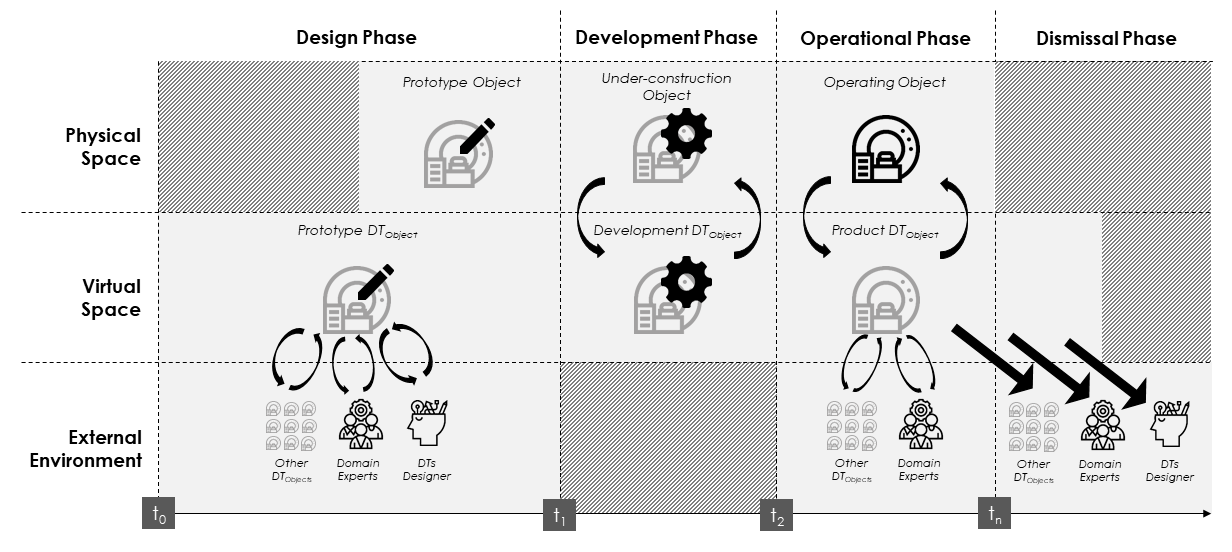
\includegraphics[width=0.9\textwidth]{images/dt_lifecycle_1.png}
    \caption[Lifecycle of a \acrshort{ct} scanner and its \acrshort{dt}, starting from the development of the \acrshort{dt}]{Lifecycle of a \acrshort{ct} scanner and its \acrshort{dt}, starting from the development of the \acrshort{dt}. From \cite{barricelliSurveyDigitalTwin2019}, \textit{Design Implications} section, CC-BY 4.0 license.}
    \label{fig:dt_lifecycle_1}
\end{figure}

For describing these two lifecycles, an example of a \acrfull{ct} scanner is used. The first lifecycle is shown in Figure~\ref{fig:dt_lifecycle_1}. The \acrshort{dt} is created before the physical object as a prototype $DT_{object}$, which helps the designers in the design phase of the prototype object. The prototype $DT_{object}$ acts as a virtual model of the real prototype, allowing the designers to simulate, test, modify, and validate their design choices using data from the prototype $DT_{object}$ and other sources. When the prototype $DT_{object}$ is done, the design phase moves to the prototype object, where the prototype $DT_{object}$ may be adjusted to address any technical issues. In the development phase, the prototype $DT_{object}$ becomes a development $DT_{object}$, which interacts with the production machines to monitor and optimize the assembly/construction of the object, i.e., its physical twin. When the object is built, the development $DT_{object}$ becomes a product $DT_{object}$, and the operational phase begins. The product $DT_{object}$ matches the object and tracks and mirrors the \acrshort{dt} scanner while it is in use. The product $DT_{object}$ also learns and adapts to the object during its operation. When the object is no longer used the dismissal phase starts, first for the object and then for the $DT_{object}$. The historical data of the product $DT_{object}$ are backed up and shared with other \acrshort{dt}s and domain experts, so that they can use the information to improve the production of future devices.

\begin{figure}
    \centering
    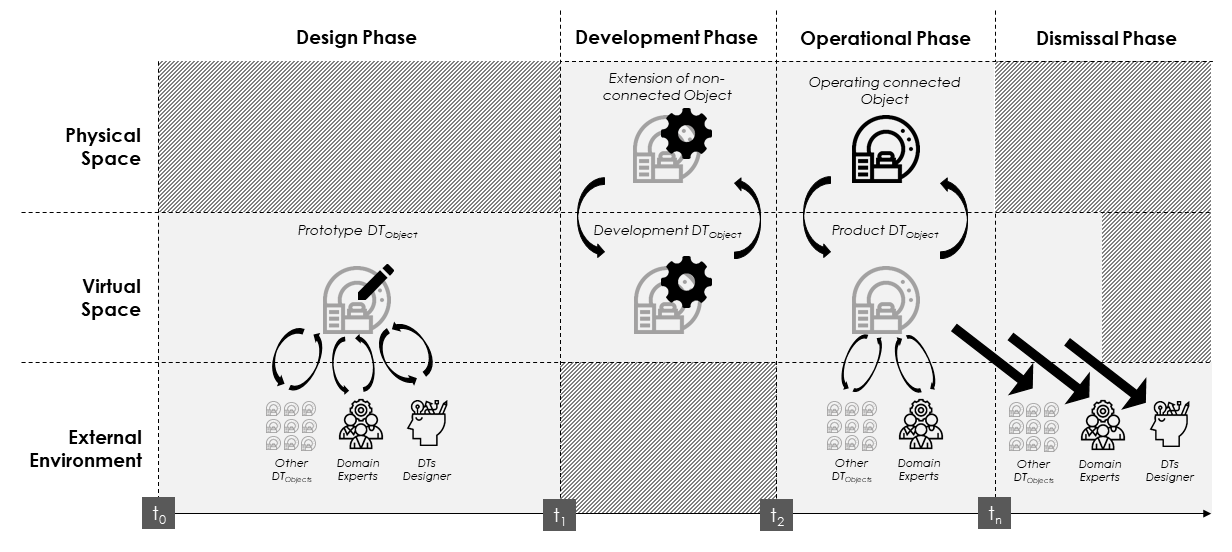
\includegraphics[width=0.9\textwidth]{images/dt_lifecycle_2.png}
    \caption[Lifecycle of a \acrshort{ct} scanner and its \acrshort{dt}, when the \acrshort{ct} scanner already exists]{Lifecycle of a \acrshort{ct} scanner and its \acrshort{dt}, when the \acrshort{ct} scanner already exists. From \cite{barricelliSurveyDigitalTwin2019}, \textit{Design Implications} section, CC-BY 4.0 license.}
    \label{fig:dt_lifecycle_2}
\end{figure}

The second lifecycle is in Figure~\ref{fig:dt_lifecycle_2}. In this case, the object is already existing and in use, but it does not have a connected DT. The design phase creates a new prototype DT ($DT_{object}$), which is tested, modified and validated. The development phase connects the existing object and the $DT_{object}$, now a development $DT_{object}$. The operational phase is the life of the two twins, the connected object and the product $DT_{object}$, which work together until their disposal in the dismissal phase. The (physical and digital) twins rely on a synergistic and continuous interaction, which enables monitoring, predicting, and optimizing all their functions.

\section{Internet of Things and Smart Homes}

An \acrfull{iot} ecosystem is defined as a set of smart devices, social networks, applications, recommender systems, and users~\parencite{barricelliDesigningEndUserDevelopment2015}. Smart objects embed electronic devices in order to allow users to interact with them: in this way users can control and use them in everyday life. For instance, the application of IoT to the smart home offers home inhabitants the possibility to control several smart objects such as lights, televisions, thermostat, shutters, locks, humidity sensors and so on~\parencite{kortuemSmartObjectsBuilding2010,wuRespectChangeUser2017}.

The term end users refers to non-technical people that do not have programming skills or knowledge about computer technologies but want to use computer systems for their daily activities (work, entertainment...).

\acrfull{eud} can be defined as “the set of methods, techniques, tools, and socio-technical environments that allow end users to act as professionals in those ICT-related domains in which they are not professionals, by creating, modifying, extending and testing digital artifacts without requiring knowledge in traditional software engineering techniques”~\parencite{barricelliEnduserDevelopmentEnduser2019}.

A smart home should be personalized to the needs of its inhabitants and, at the same time, the methods to carry out such personalization should be suitable to end users who are not software professionals. EUD approaches to personalizing the behaviour of smart homes are usually offered by web or mobile applications [4][1][18].

\subsection{Routines}

In recent years, commercial physical devices for smart home control are available on the market (e.g., Google Nest Mini, Amazon Echo Show, and Apple HomePod). Such systems allow users to control their smart devices through routines, i.e. sequences of actions that users can define on smart home control systems to be executed when specific conditions are met (i.e., at a certain time or date, when a specific event occurs, when a user invokes the routine). The routine creation is usually supported through a VA or a companion app.

Like for ecosystem creation, for routine creation there are many similarities in the way Google Home, Amazon Alexa, and Apple Home let the user operate. All applications present a predefined set of routines that can be adapted by the users. Examples of such routines are: Good morning, Bedtime, and I'm home.

The common anatomy of a routine as constituted by two main parts:
\begin{itemize}
    \item Trigger. A routine can be started in various ways:
        \begin{itemize}
            \item Voice command: the user can define one or more voice commands that trigger the routine;
            \item Time: the user can define the time of day and the day(s) of the week when the routine has to be triggered;
            \item Sunrise/sunset: the user can define the time of sunrise or sunset, or a time range around such events, and also in this case, the user can select the day(s) of the week in which the routine has to be repeated;
            \item Device: when a sensor device (e.g., smartphone GPS, movement sensor) recognizes a significant event, the routine is triggered (for example, when someone comes close to the entrance door, then the speaker announces a message).
        \end{itemize}
    \item Actions. One or more actions can be included in a routine and they can be of several types:
        \begin{itemize}
            \item Information: weather, commute information, ecc.;
            \item Reminders: calendar events, shopping list, ecc.;
            \item Announcements: send messages or reads texts;
            \item Management of connected devices: lights, electric plugs, thermostats, door locks, alarm systems;
            \item Media control: play news, music, radio, sleep sounds.
        \end{itemize}
\end{itemize}

In general, a routine is expressed as a statement composed of a condition --- WHEN something happens --- and one or more actions that are executed if the condition is met --- THEN do something.
